\documentclass[a4paper]{article}
\usepackage[14pt]{extsizes}
\usepackage[utf8]{inputenc}
\usepackage[T2A]{fontenc}
\usepackage{amssymb,amsmath,mathtext}
\usepackage{indentfirst,amsfonts}
\usepackage[english, russian]{babel}
\usepackage{setspace}
\usepackage{graphicx}
\usepackage{pscyr}
\usepackage{booktabs}
\usepackage[left=30mm, top=20mm, right=10mm, bottom=20mm, nohead, footskip=10mm]{geometry} % настройки полей документа
\usepackage{sectsty}
\usepackage{tocloft}
\renewcommand\cftsecfont{\mdseries}
\renewcommand\cftsecpagefont{\mdseries}
\graphicspath{{graphs/}}
\onehalfspacing
\renewcommand{\rmdefault}{ftm} % Times New Roman
\addto\captionsrussian{\renewcommand{\contentsname}{\normalfont Содержание}}
\addto\captionsrussian{\renewcommand{\refname}{\centering СПИСОК ИСПОЛЬЗОВАННЫХ ИСТОЧНИКОВ}}
\allsectionsfont{\normalfont}
\begin{document}
	%Титульный лист
	\begin{titlepage} % начало документа
	
	% НАЧАЛО ТИТУЛЬНОГО ЛИСТА
	\begin{center}
		\small{ФЕДЕРАЛЬНОЕ ГОСУДАРСТВЕННОЕ БЮДЖЕТНОЕ ОБРАЗОВАТЕЛЬНОЕ}\\ 
		УЧРЕЖДЕНИЕ ВЫСШЕГО ОБРАЗОВАНИЯ\\
		«МОСКОВСКИЙ ГОСУДАРСТВЕННЫЙ УНИВЕРСИТЕТ\\
		имени М.В.ЛОМОНОСОВА»\\
		\hfill \break
		%\normalsize{ФИЗИЧЕСКИЙ ФАКУЛЬТЕТ}\\
		ФИЗИЧЕСКИЙ ФАКУЛЬТЕТ \\
		\hfill \break
		КАФЕДРА МАТЕМАТИЧЕСКОГО МОДЕЛИРОВАНИЯ И ИНФОРМАТИКИ\\
		\hfill \break
		\hfill \break
		\hfill \break
		\hfill \break
		БАКАЛАВРСКАЯ РАБОТА\\
		\hfill \break
		\textbf{НЕЙРОСЕТЕВОЙ СИНТЕЗ ТЕКСТУР С ТРЕНДАМИ}\\
	\end{center}
	
	\hfill \break

	\begin{flushright}
		Выполнил студент \\
		435 группы:\\
		Будакян Я. С.\\
		\underline{\hspace{3cm}}\\
		\hfill \break
		Научный руководитель: \\
		к.т.н., доц. Грачев Е. А.\\
		\underline{\hspace{3cm}}
	\end{flushright}
	
	\begin{flushleft}
		Допущена к защите\\
		Зав. кафедрой \underline{\hspace{3cm}}\\
	\end{flushleft}
	\hfill \break
	\begin{center}
		Москва \\
		\hfill \break
		2017 
	\end{center}
	
	\thispagestyle{empty} % выключаем отображение номера для этой страницы
	
	% КОНЕЦ ТИТУЛЬНОГО ЛИСТА

\end{titlepage}  % КОНЕЦ ДОКУМЕНТА !
	%Учет титульного листа в нумерации
	\setcounter{page}{2}
	\tableofcontents
	\addcontentsline{toc}{section}{ВВЕДЕНИЕ}
	% ВВЕДЕНИЕ
	\clearpage
\section*{\hfil ВВЕДЕНИЕ \hfil}
	В современной добыче полезных ископаемых активно применяются средства математического моделирования для симуляции процессов, происходящих в пласте. Однако, на данный момент полноценное моделирование не представляется возможным, поэтому используются различные приближенные методы. Для правильной симуляции процессов, происходящих в недрах, необходимо смоделировать саму среду, в которой эти процессы протекают. Обычно, данные о структуре среды доступны только в некотором количестве точек (скважин), в которых непосредственно идет добыча. Предлагается попытаться использовать методы машинного обучения для синтеза модели среды, похожей на природную. В рамках решения этой проблемы возникает задача синтеза текстур с трендами, например, для учета каких-либо пространственных корреляций. 
	
	Под текстурой с трендом в данном случае понимается изображение, в котором есть изменение некоторой статистической характеристики вдоль одного из направлений. Такими характеристиками, например, могут быть изменение интенсивности появления частиц среды или пористости среды.
	
	Базовым подходом в задаче синтеза текстур на данный момент является использование искусственных нейросетей. Однако, известные работы в области синтеза текстур с помощью искусственных нейросетей \cite{texture-synthesis-using-CNN, texture-networks} показывают, что у нейросетевых моделей есть проблемы с воспроизведением формы объектов, а также различных пространственно скоррелированных структур. Соответственно, целью данной работы ставится поиск нейросетевой архитектуры, способной улавливать и воспроизводить протяженные корреляции.
	
	Для упрощения задачи, будем в дальнейшем рассматривать множество изображений с трендами, удовлетворяющее следующим ограничениям:
	
	\begin{itemize}
		\item Это монохромные изображения 256 x 256 пикселей
		\item Изменяющимся свойством является интенсивность появления частиц $\lambda$
		\item Тренд является линейным и направлен вдоль оси изображения $z_1$: 
		$ \lambda = \lambda_{init} + k z_1 $
		\item По оси $z_2$ остается равномерное распределение частиц
	\end{itemize}
	
	Каждый такой тренд фиксируется значениями $\lambda_{init}$ и $\lambda_{final}$. Следовательно, 
	$$k = \frac{\lambda_{final} - \lambda_{init}}{256}$$
	Пример такого изображения с трендом интенсивности приведен на (Рис. \ref{1-trend-example}):
	
	\begin{figure}[h]
		\centering{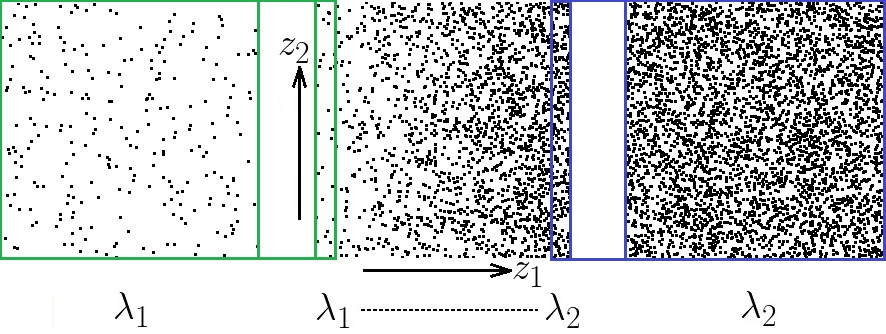
\includegraphics[width=\linewidth]{1-introduction/trend-example}}
		\caption{Пример изображения с трендом, фиксируемого двумя изображениями}
		\label{1-trend-example}
	\end{figure}
	
	Математически сформулировать постановку описанной задачи можно с помощью так называемой вероятностной постановки задачи обучения \cite{Voron-ML, GAN-original}.
	
	Рассмотрим многомерное пространство $X$, содержащее множество всех изображений $x$: $X = \{x\}$. Пусть у нас есть обучающая выборка из изображений, содержащих в себе рассматриваемое множество трендов $D = \{x_i\}$. Тогда считается, что  обучающая выборка изображений с трендами $D$ задает в этом пространстве вероятностное распределение $P_X : X \longrightarrow [0,1]$, устроенное таким образом, что точки, соответствующие изображениям из выборки, имеют высокую вероятность, а остальные - низкую. Таким образом, с математической точки зрения задача синтеза текстуры с трендом сводится к синтезу случайного изображения $x'$, принадлежащего распределению, близкому к задаваемому обучающей выборкой:
	$$ P_{X'} \approx P_X, \quad x' \sim X'$$
	
	``Классический'' статистический подход к решению подобного рода задач заключается в введении в рассмотрение параметризированного семейства распределений вероятности и его подстройке к имеющимся данным:
	
	\begin{itemize}
		\item Вводится параметризированное семейство распределений вероятности $P_{\theta}(x)$
		\item Параметры $\theta$ находятся из обучающей выборки:
		$$ \mathcal{L}_{\theta}(D) = \prod_{x \in D} P_{\theta}(x) $$
		$$ \theta^{*} = \underset{\theta}{\arg\max} \mathcal{L}_{\theta}(D)$$
		\item Генерируется объект (изображение) из распределения $ P_{\theta^{*}}$
	\end{itemize}
	
	Этот подход приводит к проблемам:
	
	\begin{itemize}
		\item Пространство параметров $\theta$ может быть огромной размерности
		\item Известной параметрической модели распределения может вообще не существовать
	\end{itemize}
	
	Простой пример объекта со сложным пространством параметров - человеческое лицо. Задачу генерации изображения реалистичного человеческого лица долгое время не могли решить с удовлетворительным качеством. Однако последние достижения в области искусственных нейронных сетей привели к существенному улучшению качества генеративных моделей самого разнообразного типа. В частности, впечатляющие результаты были достигнуты с помощью генеративных состязательных сетей (GAN) \cite{cGAN, cGAN-face, EBGAN, BEGAN}, что мотивирует попытку применения нейросетей этой архитектуры в поставленной задаче.
	
	\subsection*{Постановка задачи}
	
	Таким образом, для достижения обозначенной во введении цели, поставить задачу работы можно так:
	
	\begin{itemize}
		\item Разработать модифицированные для синтеза описанного множества текстур с трендами архитектуры GAN
		\item Провести вычислительные эксперименты, связанные с обучением нейросетей (то есть, с решением задач многопараметрической оптимизации)
		\item Синтезировать с помощью обученных нейросетей новые текстуры и верифицировать их
	\end{itemize}
	% Нейронные сети
	\clearpage
\section{Нейронные сети}
	В общем смысле, искусственная нейронная сеть - это математическая модель, построенная по принципу организации и функционирования биологических нейронных сетей. Она представляет из себя систему соединенных простых блоков - искусственных нейронов, каждый из которых имеет входы и выходы для взаимодействия с другими нейронами. Главное преимущество нейронных сетей перед традиционными алгоритмами в том, что они обучаются на некотором наборе данных, а не программируются в классическом смысле этого понятия. Процесс обучения заключается в нахождении оптимальных весовых коэффициентов между нейронами. С математической точки зрения, процесс обучения - это задача многопараметрической нелинейной оптимизации.
	\subsection{Математическая модель нейрона}
		Одиночный нейрон обычно представляет собой взвешенный сумматор с нелинейной функцией активации на выходе:
		$$x_{out} = \phi(\vec{w} \cdotp \vec{x_{in}}),$$
		где $\vec{w}$ - вектор весовых коэффициентов связей, $\vec{x_{in}}$ - входной вектор, $\phi$ - нелинейная функция активации (Рис. \ref{3-artificial-neuron-model}).
		
		\begin{figure}[h]
			\centering{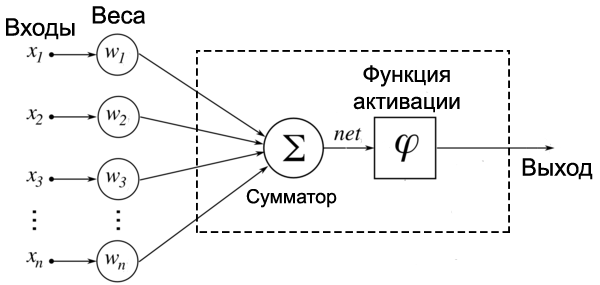
\includegraphics[width=0.9\linewidth]{3-ann/artificial-neuron-model}}
			\caption{Математическая модель нейрона}
			\label{3-artificial-neuron-model}
		\end{figure}
		
		Функция активации может выбираться разной в зависимости от задачи. Наиболее часто используемые функции:
		
		\begin{itemize}
			\item Сигмоида (логистическая функция)
					$$\sigma(x) = \frac{1}{1 + e^{-x}}$$
			\item Гиперболический тангенс
			\item ReLU
					$$ReLU(x) = \max(0, x)$$
			\item softmax
					$$\sigma(\vec{x})_j = \frac{e^{x_j}}{\sum_{k=1}^{N} e^{z_k}}$$
		\end{itemize}
		Множество таких нейронов объединяется в сеть и обучается каким-либо методом оптимизации.
	\subsection{Метод обратного распространения ошибки}
		Метод обратного распространения ошибки (backpropagation) - самый широко используемый и успешный алгоритм обучения глубоких (многослойных) нейронных сетей. Суть этого метода заключается в распространении сигналов ошибки от выходов сети к ее входам в обратном к распространению сигнала в сети направлении. Это позволяет вычислить производные ошибки по весам сети, которые потом можно использовать в любом градиентном алгоритме оптимизации (например, в стохастическом градиентном спуске).
		
		Обозначим множество входов сети как $\{x_1, \ldots, x_n\}$, множество выходов - $O$, $w_{ij}$ - вес, присвоенный ребру, соединяющему $i$-й и $j$-й узлы, $y_k$ - известные (правильные) ответы, $o_i$ - выход $i$-го узла. Введем функцию ошибки (например, сумма квадратов расстояний):
		$$ L(\vec{x}, W) = \frac{1}{2} \sum_{k \in O} (y_k - o_k)^2, $$
		где $W = \{w_{ij}\}$ - матрица весовых коэффициентов
		
		Рассмотрим сначала нейроны последнего слоя. Весовой коэффициент $w_{ij}$ влияет на выход сети как часть суммы $S_j = \sum_i w_{ij} x_i$. Соответственно,
		$$ \frac{\partial L}{\partial w_{ij}} = \frac{\partial L}{\partial S_j} \frac{\partial S_j}{\partial w_{ij}} = x_i \frac{\partial L}{\partial S_j} $$
		
		Аналогично, $S_j$ влияет на общую ошибку только в рамках выхода $j$-го узла $o_j$, поэтому
		$$ \frac{\partial L}{\partial S_j} = \frac{\partial L}{\partial o_j} \frac{\partial o_j}{\partial S_j}  = (\frac{\partial}{\partial o_j} \frac{1}{2} \sum_{k \in Out} (y_k - o_k)^2)(\frac{\partial \phi(S)}{\partial S} \bigg|_{S = S_j})$$
		Если узел $j$ не находится на последнем слое, то у него есть набор связей с нейронами следующего слоя. Обозначим их множество как $K_j$. Тогда
		$$ \frac{\partial L}{\partial S_j} = \sum_{k \in K_j} \frac{\partial L}{\partial S_k} \frac{\partial S_k}{\partial S_j} $$
		$$ \frac{\partial S_k}{\partial S_j} = \frac{\partial S_k}{\partial o_j} \frac{\partial o_j}{\partial S_j} = w_{jk}\frac{\partial o_j}{\partial S_j} $$
		$ \frac{\partial L}{\partial S_k}$ - аналогичная поправка, но для нейрона следующего слоя. В итоге, получены выражения для производных ошибки по весам для нейронов выходного слоя, а аналогичные производные для нейронов внутренних слоев выражены через нейроны следующих слоев. Это и есть процесс обратного распространения ошибки - градиенты ошибки по весам вычисляются последовательно, начиная с выходного слоя и заканчивая первым.
	\subsection{Сверточные нейронные сети}
		Сверточные нейронные сети (CNN - convolutional neural networks)- это специальная архитектура нейронной сети, нацеленная на эффективное распознавание изображений, впервые предложенная Яном Лекуном \cite{CNN-original}. Структура такой сети имеет некоторое сходство со строением зрительной коры головного мозга. Свое название CNN получили из-за наличия сверточных слоев, в которых каждый фрагмент изображения умножается на ядро свертки, полученный результат суммируется и записывается в аналогичную позицию выходного изображения. Одно отдельное ядро свертки обычно интерпретируют как кодирование какого-либо признака изображения. При этом сами ядра выучиваются сетью самостоятельно, а не закладываются человеком. В CNN чередуются сверточные слои и субдискретезирующие слои, таким образом более глубокие сверточные слои могут выделять абстрактные детали изображения, вплоть до общих понятий, таких как "кошка", "собака", и т.п. На данный момент CNN считаются базовым нейросетевым подходом при работе с изображениями.
	\subsection{Генеративные состязательные сети}
		Архитектура нейронной сети, получившая название генеративной состязательной сети (generative adversarial network - GAN), впервые была описана в 2014 году \cite{GAN-original}. За последнее время сети такого типа добились больших успехов в задачах синтеза объектов из сложных распределений. Этим объясняется мотивация попытки применения данной архитектуры для решения поставленной задачи.
		\subsubsection{Общая структура}
			Переформулируем изначальную задачу нахождения такой процеруды синтеза $X'$, что $ P_{X'} \approx P_X$:
			$$ \rho(P_{X'}, P_X) \longrightarrow \underset{P_{X'}}{\min} $$
			Введем параметризированную процедуру генерации:
			$$ X' = g_{\theta}(\cdot) $$
			Получаем:
			$$ \rho(P_{X'}, P_X) \longrightarrow \underset{P_{X'}}{\min} $$
			$$ \rho(g_{\theta}(\cdot), P_X) \longrightarrow \underset{g_{\theta}(\cdot)}{\min} $$
			$$ \rho(g_{\theta}(\cdot), P_X) \longrightarrow \underset{\theta}{\min} $$
			Возникает вопрос: что использовать в качестве метрики похожести двух распределений $\rho$, где одно из распределений задано обучающей выборкой.
			В качестве такой метрики можно использовать функцию потерь обученного классификатора, потому что естественно предположить, что чем чаще ошибается обученный классификатор, тем больше одно распределение похоже на другое. Тогда задача примет вид:
			$$ \rho(P_{X'}, P_X) \longrightarrow \min \Leftrightarrow L \longrightarrow \max, $$
			где $L$ - функция потерь обученного классификатора.
			Соответственно, можно ввести две нейросети:
	
			\begin{itemize}
				\item $d_{\zeta}(x)$ - классификатор для измерения расстояния, ``дискриминатор''
				\item $g_{\theta}(x)$ - сеть, трансформирующая шум в $X'$, ``генератор''
			\end{itemize}
	
			Суть использования двух сетей состоит в том, что они обучаются совместно, конкурируя друг с другом: генератор пытается имитировать целевое распределение, а дискриминатор пытается классифицировать поступающие от генератора и из обучающей выборки изображения на 2 класса: реальные (из изначального распределения $P_X$) и ложные (из $P_{X'}$, т.е. произведенные генератором).
			Для дальнейшего рассмотрения введем функцию потерь дискриминатора(например, logloss):
			$$ l_1 = l(d_{\zeta}(x), 1) \text{ - ошибка 1 рода} $$
			$$ l_2 = l(d_{\zeta}(x'), 0) \text{ - ошибка 2 рода}$$
			$$ L(X, X') = \frac{1}{2} \mathbb{E}_{X} l_1 + \frac{1}{2} \mathbb{E}_{X'} l_2 = -\frac{1}{2} (\mathbb{E}_{X} \log d_{\zeta}(x) + \mathbb{E}_{X'} \log (1 - d_{\zeta}(x'))) = $$
			$$ =  -\frac{1}{2} (\mathbb{E}_{X} \log d_{\zeta}(x) + \mathbb{E}_{V} \log (1 - d_{\zeta}(g_{\theta}(v)))) = L(\zeta, \theta) .$$
			Функция потерь обученного классификатора:
			$$ L^*(\theta) = \underset{\zeta}{\min} L(\zeta, \theta) $$
			Соответственно,
			$$ \underset{\zeta}{\min} L(\zeta, \theta) \longrightarrow \underset{\theta}{\max} $$
			$$ \theta^* = \underset{\theta}{\arg\max} \left[ \underset{\zeta}{\min} L(\zeta, \theta) \right] $$
			Определим оптимальный дискриминатор:
			$$ d^*_{\theta} = d_{\zeta^*(\theta)} $$
			$$ \zeta^*(\theta) =  \underset{\zeta}{\arg\min} L(\zeta, \theta)$$
		\subsubsection{Обучение GAN}
			Итак, задача обучения GAN свелась к нахождению
			$$ \theta^* = \underset{\theta}{\arg\max} \left[ \underset{\zeta}{\min} L(\zeta, \theta) \right] $$
			В итоге, процесс обучения принимает следующий вид:
	
			\begin{itemize}
				\item Обучаем дискриминатор при фиксированном генераторе
				\item Обучаем генератор при фиксированном дискриминаторе
				\item Повторяем до сходимости параметров обеих моделей
			\end{itemize}
			Описанный процесс схематично изображен на (Рис. \ref{5-gan-training}).
	
			\begin{figure}[h!]
				\centering{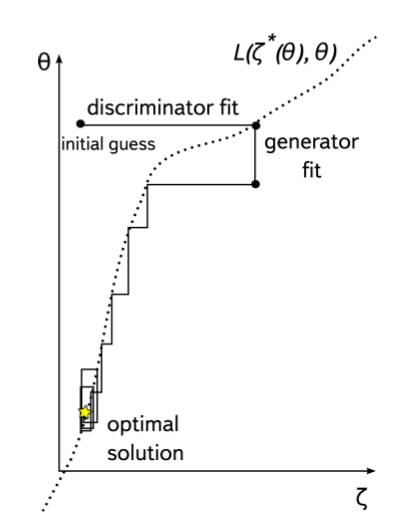
\includegraphics[width=0.4\linewidth]{5-GAN/gan-training}}
				\caption{Схематическое изображение процесса обучения GAN.}
				\label{5-gan-training}
			\end{figure}
	
		\subsubsection{Модификация ``pix2pix GAN''}
			Для решения задачи была опробована модификация обычной структуры GAN под названием ``pix2pix GAN'' \cite{pix2pix, p2p-vessnet}. Ее отличие от схемы GAN, введенной выше, состоит в том, что вместо шума на вход генератору приходят другие изображения, на которых он основывается при синтезе. Схематически ее устройство изображено на (Рис. \ref{5-p2p}).
	
			\begin{figure}[h!]
				\centering{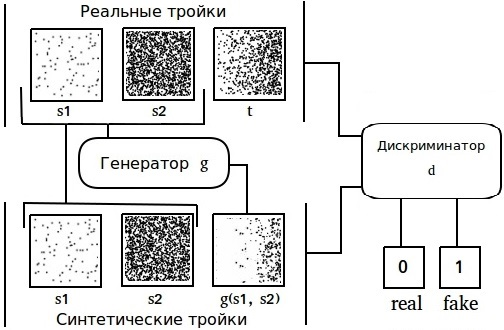
\includegraphics[width=0.75\linewidth]{5-GAN/p2p}}
				\caption{Схематическое устройство сети pix2pix GAN.}
				\label{5-p2p}
			\end{figure}
	
			Для pix2pix сети общий функционал потерь выглядит следующим образом: $$ L(G, D) = L_{adv}(G, D) + \eta L1$$
			$$L1 = \mathbb{E}_{p_{data}(s_1, s_2, r)} (\parallel r - G(s_1, s_2) \parallel_1)$$
			$$ L_{adv}(G, D) = \mathbb{E}_{p_{data}(s_1, s_2, r)}\log D(s_1, s_2, r) +  \mathbb{E}_{p_{data}(s_1, s_2)} \log (1 - D(s_1, s_2, G(s_1, s_2)))$$
			где G, D - генератор и дискриминатор, $(s_1, s_2, r)$ - тройка изображений (интенсивность слева, справа и реальное изображение с трендом),  $\mathbb{E}_{p_{data}(s_1, s_2, r)}$ - мат. ожидание логарифмического правдоподобия того, что тройка изображений $(s_1, s_2, r)$ принадлежит вероятностному распределению реальных троек $p_{data}(s_1, s_2, r)$, а $p_{data}(s_1, s_2)$ соответствует распределению реальных изображений $s_1, s_2$.
	
			В качестве генератора в \cite{pix2pix, p2p-vessnet} использовалась сеть ``U-Net'' \cite{unet}. Основное отличие сети ``U-Net'' от обычной сети архитектуры ``encoder-decoder'' заключается в наличии прямых связей между сверточными и разверточными слоями. Использование такого типа генератора позволяло увеличить качество синтезируемых изображений. Схемы сетей типа ``U-Net'' и ``Encoder-decoder'' приведены на (Рис. \ref{5-unet-sheme}).
			
			\begin{figure}[h!]
				\centering{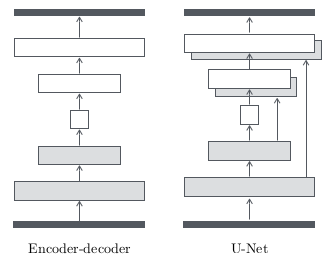
\includegraphics[width=0.65\linewidth]{5-GAN/unet-encoder}}
				\caption{Схематическое изображение нейросети-генератора.}
				\label{5-unet-sheme}.
			\end{figure}
	% Стохастическая оптимизация
	\section{Методы стохастической оптимизации}
	Для обучения глубоких нейросетей применяется метод обратного распространения ошибки, который позволяет расчитать градиенты весов, и различные методы стохастической оптимизации первого порядка. В данной работе для обучения моделей применялось 2 алгоритма оптимизации под названиями "RMSprop" и "Adam".
	\subsection{RMSprop}
	\subsection{Adam}
	
	% TR-MSE
	\clearpage
\section{Оценка качества синтеза текстур с трендом}
	После обучения сети, необходимо проверить, что сгенерированные ей изображения действительно имеют искомые характеристики (то есть, содержат искомый тренд). Для этого вводится специальная метрика, которая будет учитывать наличие в изображении тренда интенсивности частиц. Рассмотрим среднюю плотность черных пикселей в некотором окне $\xi_k$, и пройдем этим окном по изображению.
	$$\xi_k = \frac{1}{H w}{\sum_{i=k}^{k+w} \sum_{j=0}^{H}\left| \frac{x(i, j) - 255}{255} \right|}, $$$$k = \overline{1, W - w} $$
	
	Построив график $\xi(k)$, можно увидеть, как меняется плотность черных пикселей и прослеживается ли тренд (Рис. \ref{7-window}).
	
	\begin{figure}[h!]
		\centering{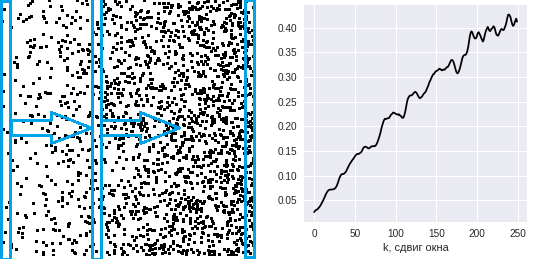
\includegraphics[width=0.75\linewidth]{7-verification/window}}
		\caption{Прохождение окном, W, H - размеры изображения, w - ширина окна.}
		\label{7-window}
	\end{figure}
	
	В качестве метрики можно взять среднеквадратичную ошибку:
	$$ \xi = \frac{K}{W-w}\sum_{k=1}^{W-w} (\xi_k - \xi_{0k})^2,$$
	где $\xi_{0k}$ - это $\xi_k$, усредненное по изображениям, содержащим истинный тренд, а $K$ - нормировочный множитель, вводимый для того, чтобы метрики сетей, обученных на разных выборках можно было сравнивать между собой. Соответственно, чем меньше значение метрики, тем лучше тренд, присутствующий на сгенерированном изображении, приближает искомый.
	% Результаты
	\clearpage
\section{Результаты вычислительных экспериментов}
	Архитектуры, описанные в пункте 1.4.3, были реализованы в виде компьютерных программ на языке Python с помощью библиотеки для построения искусственных нейронных сетей Keras \cite{keras}, которая, в свою очередь, использует для расчетов пакет Tensorflow \cite{tf}. Использованные версии программных пакетов указаны в Приложении 1. Обучение проводилось на синтетических данных, сгенерированных самостоятельно реализованным генератором. 
	\subsection{Выборки с реализацией одного тренда}
		\subsubsection{Выборка 1}
			% sand:trend 2
			Выборка состояла из 3000 обучающих изображений и 500 валидационных. Частицами среды были круги диаметром 7 пикселей. Все изображения содержали в себе различные случайные реализации одного тренда интенсивности
			$$\lambda(x) = 0.2 + 0.01875x : \lambda_i = 0.2, \quad \lambda_f = 5$$
			
			Отличия в параметрах нейросетей указаны в (Таб. \ref{8-sand-trend2-nns}). Для всех обученных моделей параметр $\eta$, отвечающий за баланс между $L_{adv}$ и $L1$, был равен 100.
			
			\begin{table}[h!]
				\begin{center}
					\begin{tabular}{|c|c|c|}
						\hline
						Сеть & Число фильтров на первом слое & Сеть-генератор \\
						\hline
						nf8 & 8 & U-Net \\
						\hline
						nf16 & 16 & U-Net \\
						\hline
						nf16woU & 16 & Encoder-decoder \\
						\hline
						nf32 & 32 & U-Net \\
						\hline
					\end{tabular}
					\caption{Отличия в параметрах моделей (Выборка 1)}
					\label{8-sand-trend2-nns}
				\end{center}
			\end{table}
			
			Примеры синтеза, полученные с помощью нейросетей с различными параметрами, приведены в (Таб. \ref{8-dataset1-images}).
			
			\begin{table}[h!]
				\begin{center}
					\begin{tabular}{p{2cm} p{2cm} p{2cm} p{2cm} p{2cm} p{2cm} p{2cm}}
						\toprule
						Вход 1 & Вход 2 & Тренд & Сеть nf8 & nf16 & nf16woU & nf32 \\
						\cmidrule(r){1-1}\cmidrule(lr){2-2}\cmidrule(lr){3-3}\cmidrule(lr){4-4}\cmidrule(lr){5-5}\cmidrule(lr){6-6}\cmidrule(l){7-7}
						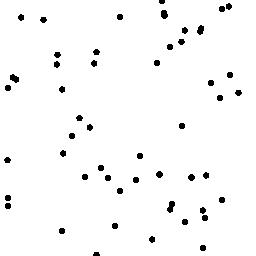
\includegraphics[width=1\linewidth]{8-results/sand-trend2/left1}
						&
						
\includegraphics[width=1\linewidth]{8-results/sand-trend2/right1}
						&
						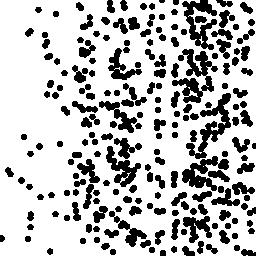
\includegraphics[width=1\linewidth]{8-results/sand-trend2/pan1}
						&
						
\includegraphics[width=1\linewidth]{8-results/sand-trend2/nf8/gen1}
						&
						
\includegraphics[width=1\linewidth]{8-results/sand-trend2/nf16/gen1}
						&
						
\includegraphics[width=1\linewidth]{8-results/sand-trend2/nf16_woUnet/gen1}
						&
						
\includegraphics[width=1\linewidth]{8-results/sand-trend2/nf32/gen1}
						\\
						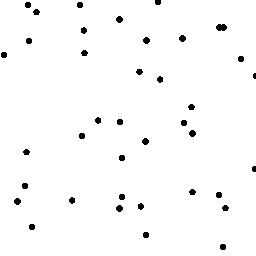
\includegraphics[width=1\linewidth]{8-results/sand-trend2/left2}
						&
						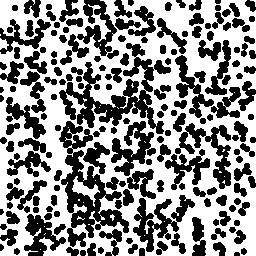
\includegraphics[width=1\linewidth]{8-results/sand-trend2/right2}
						&
						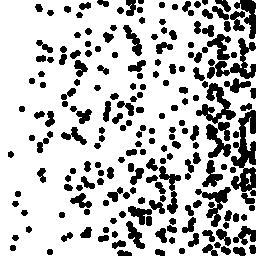
\includegraphics[width=1\linewidth]{8-results/sand-trend2/pan2}
						&
						
\includegraphics[width=1\linewidth]{8-results/sand-trend2/nf8/gen2}
						&
						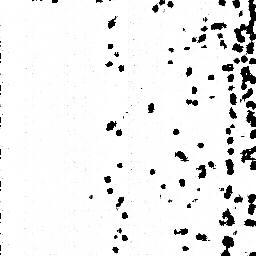
\includegraphics[width=1\linewidth]{8-results/sand-trend2/nf16/gen2}
						&
						
\includegraphics[width=1\linewidth]{8-results/sand-trend2/nf16_woUnet/gen2}
						&
						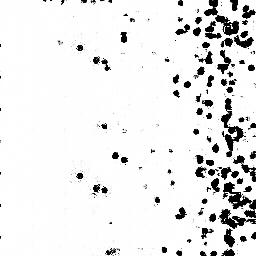
\includegraphics[width=1\linewidth]{8-results/sand-trend2/nf32/gen2}
						\\
						
\includegraphics[width=1\linewidth]{8-results/sand-trend2/left3}
						&
						
\includegraphics[width=1\linewidth]{8-results/sand-trend2/right3}
						&
						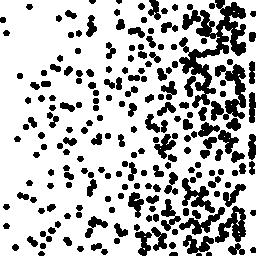
\includegraphics[width=1\linewidth]{8-results/sand-trend2/pan3}
						&
						
\includegraphics[width=1\linewidth]{8-results/sand-trend2/nf8/gen3}
						&
						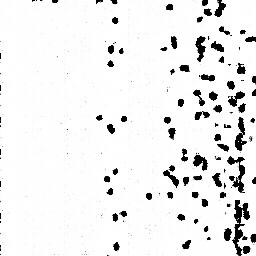
\includegraphics[width=1\linewidth]{8-results/sand-trend2/nf16/gen3}
						&
						
\includegraphics[width=1\linewidth]{8-results/sand-trend2/nf16_woUnet/gen3}
						&
						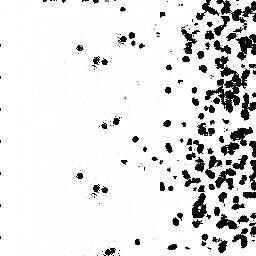
\includegraphics[width=1\linewidth]{8-results/sand-trend2/nf32/gen3}
						\\
						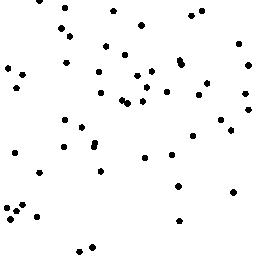
\includegraphics[width=1\linewidth]{8-results/sand-trend2/left4}
						&
						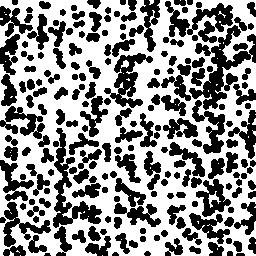
\includegraphics[width=1\linewidth]{8-results/sand-trend2/right4}
						&
						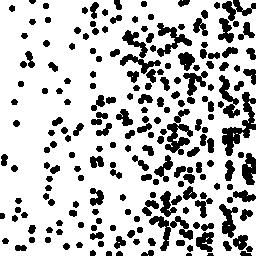
\includegraphics[width=1\linewidth]{8-results/sand-trend2/pan4}
						&
						
\includegraphics[width=1\linewidth]{8-results/sand-trend2/nf8/gen4}
						&
						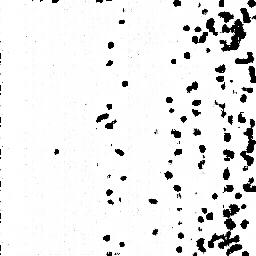
\includegraphics[width=1\linewidth]{8-results/sand-trend2/nf16/gen4}
						&
						
\includegraphics[width=1\linewidth]{8-results/sand-trend2/nf16_woUnet/gen4}
						&
						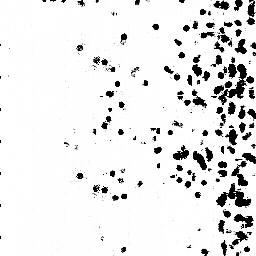
\includegraphics[width=1\linewidth]{8-results/sand-trend2/nf32/gen4}
						\\
						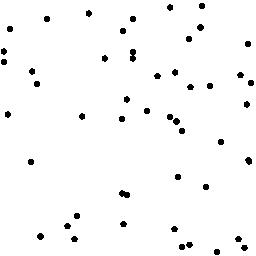
\includegraphics[width=1\linewidth]{8-results/sand-trend2/left5}
						&
						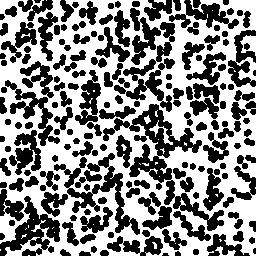
\includegraphics[width=1\linewidth]{8-results/sand-trend2/right5}
						&
						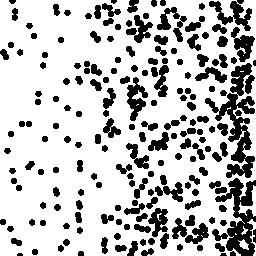
\includegraphics[width=1\linewidth]{8-results/sand-trend2/pan5}
						&
						
\includegraphics[width=1\linewidth]{8-results/sand-trend2/nf8/gen5}
						&
						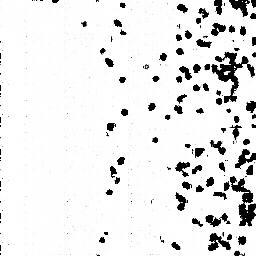
\includegraphics[width=1\linewidth]{8-results/sand-trend2/nf16/gen5}
						&
						
\includegraphics[width=1\linewidth]{8-results/sand-trend2/nf16_woUnet/gen5}
						&
						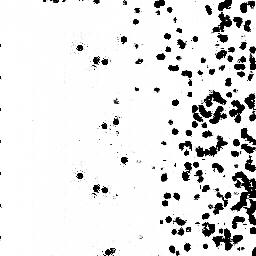
\includegraphics[width=1\linewidth]{8-results/sand-trend2/nf32/gen5}
						\\
						\hline
					\end{tabular}
					\caption{Примеры синтеза (Выборка 1)}
					\label{8-dataset1-images}
				\end{center}
			\end{table}
			
			\break
			
			График приближения тренда различными сетями показан на (Рис. \ref{8-sand-trend2-results}).
			
			\begin{figure}[h!]
				\centering{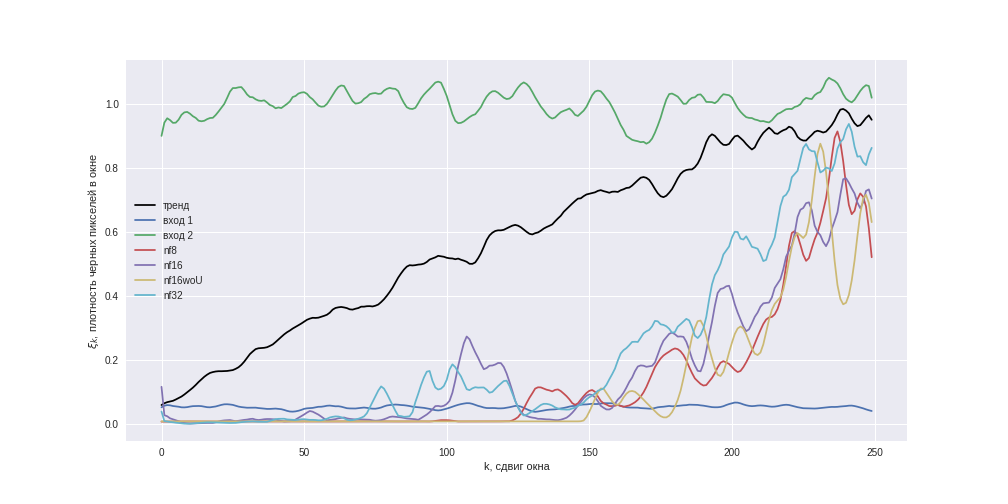
\includegraphics[width=\linewidth]{8-results/sand-trend2/results}}
				\caption{Аппроксимация тренда различными сетями (Выборка 1)}
				\label{8-sand-trend2-results}
			\end{figure}
			
			Значения введенной метрики для различных сетей указаны в (Таб. \ref{8-sand-trend2-metrics}).
			
			\begin{table}[h!]
				\begin{center}
					\begin{tabular}{|c|c|}
						\hline
						Сеть & Метрика \\
						\hline
						nf16woU & 0.24048\\
						\hline
						nf8 & 0.22511\\
						\hline
						nf16 & 0.18844\\
						\hline
						nf32 & 0.14589\\
						\hline
					\end{tabular}
					\caption{Значения метрики для разных сетей (меньше - лучше)}
					\label{8-sand-trend2-metrics}
				\end{center}
			\end{table}
			
			Лучшей по введенной метрике оказалась сеть nf32.
		\subsubsection{Выборка 2}
			% sand:trend 8
			Выборка состояла из 6000 обучающих изображений и 316 валидационных. Частицами среды были квадраты стороной 3 пикселя. Все изображения содержали в себе различные случайные реализации одного тренда интенсивности
			$$\lambda(x) = 1 + 0.0546875x: \lambda_i = 1, \quad \lambda_f = 15$$
			
			Отличия в параметрах обученных нейросетей указаны в (Таб. \ref{8-sand-trend8-nns}). Во всех обученных моделях в качестве сети-генератора использовалась сеть ``U-Net''.
			
			\begin{table}[h!]
				\begin{center}
					\begin{tabular}{|c|c|c|c|}
						\hline
						Сеть & Число фильтров на первом слое & $\eta$ & Метод оптимизации\\
						\hline
						nf32e5 & 32 & 5 & Adam \\
						\hline
						nf64e1 & 64 & 1 & RMSprop \\
						\hline
						nf64e5 & 64 & 5 & RMSprop \\
						\hline
						nf64e10 & 65 & 10 & RMSprop \\
						\hline
					\end{tabular}
					\caption{Отличия в параметрах моделей (Выборка 2)}
					\label{8-sand-trend8-nns}
				\end{center}
			\end{table}
			
			Примеры синтеза, полученные с помощью нейросетей с различными параметрами, приведены в (Таб. \ref{8-dataset2-images}).
			\begin{table}[h!]
				\begin{center}
					\begin{tabular}{p{2cm} p{2cm} p{2cm} p{2cm} p{2cm} p{2cm} p{2cm}}
						\toprule
						Вход 1 & Вход 2 & Тренд & Сеть nf32e5 & nf64e1 & nf64e5 & nf64e10 \\
						\cmidrule(r){1-1}\cmidrule(lr){2-2}\cmidrule(lr){3-3}\cmidrule(lr){4-4}\cmidrule(lr){5-5}\cmidrule(lr){6-6}\cmidrule(l){7-7}
						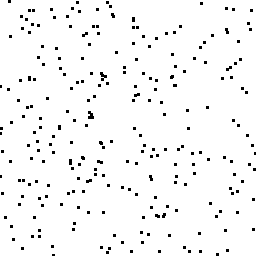
\includegraphics[width=1\linewidth]{8-results/sand-trend8/left1}
						&
						
\includegraphics[width=1\linewidth]{8-results/sand-trend8/right1}
						&
						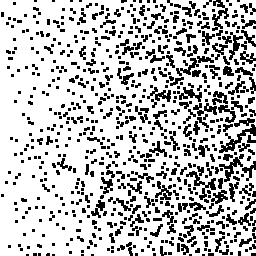
\includegraphics[width=1\linewidth]{8-results/sand-trend8/pan1}
						&
						
\includegraphics[width=1\linewidth]{8-results/sand-trend8/nf32e5/gen1}
						&
						
\includegraphics[width=1\linewidth]{8-results/sand-trend8/nf64e1/gen1}
						&
						
\includegraphics[width=1\linewidth]{8-results/sand-trend8/nf64e5/gen1}
						&
						
\includegraphics[width=1\linewidth]{8-results/sand-trend8/nf64e10/gen1}
						\\
						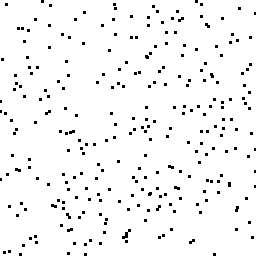
\includegraphics[width=1\linewidth]{8-results/sand-trend8/left2}
						&
						\includegraphics[width=1\linewidth]{8-results/sand-trend8/right2}
						&
						\includegraphics[width=1\linewidth]{8-results/sand-trend8/pan2}
						&
						\includegraphics[width=1\linewidth]{8-results/sand-trend8/nf32e5/gen2}
						&
						\includegraphics[width=1\linewidth]{8-results/sand-trend8/nf64e1/gen2}
						&
						\includegraphics[width=1\linewidth]{8-results/sand-trend8/nf64e5/gen2}
						&
						\includegraphics[width=1\linewidth]{8-results/sand-trend8/nf64e10/gen2}
						\\
						\includegraphics[width=1\linewidth]{8-results/sand-trend8/left3}
						&
						\includegraphics[width=1\linewidth]{8-results/sand-trend8/right3}
						&
						\includegraphics[width=1\linewidth]{8-results/sand-trend8/pan3}
						&
						\includegraphics[width=1\linewidth]{8-results/sand-trend8/nf32e5/gen3}
						&
						\includegraphics[width=1\linewidth]{8-results/sand-trend8/nf64e1/gen3}
						&
						\includegraphics[width=1\linewidth]{8-results/sand-trend8/nf64e5/gen3}
						&
						\includegraphics[width=1\linewidth]{8-results/sand-trend8/nf64e10/gen3}
						\\
						\includegraphics[width=1\linewidth]{8-results/sand-trend8/left4}
						&
						\includegraphics[width=1\linewidth]{8-results/sand-trend8/right4}
						&
						\includegraphics[width=1\linewidth]{8-results/sand-trend8/pan4}
						&
						\includegraphics[width=1\linewidth]{8-results/sand-trend8/nf32e5/gen4}
						&
						\includegraphics[width=1\linewidth]{8-results/sand-trend8/nf64e1/gen4}
						&
						\includegraphics[width=1\linewidth]{8-results/sand-trend8/nf64e5/gen4}
						&
						\includegraphics[width=1\linewidth]{8-results/sand-trend8/nf64e10/gen4}
						\\
						\includegraphics[width=1\linewidth]{8-results/sand-trend8/left5}
						&
						\includegraphics[width=1\linewidth]{8-results/sand-trend8/right5}
						&
						\includegraphics[width=1\linewidth]{8-results/sand-trend8/pan5}
						&
						\includegraphics[width=1\linewidth]{8-results/sand-trend8/nf32e5/gen5}
						&
						\includegraphics[width=1\linewidth]{8-results/sand-trend8/nf64e1/gen5}
						&
						\includegraphics[width=1\linewidth]{8-results/sand-trend8/nf64e5/gen5}
						&
						\includegraphics[width=1\linewidth]{8-results/sand-trend8/nf64e10/gen5}
						\\
						\hline
					\end{tabular}
					\caption{Примеры синтеза (Выборка 2)}
					\label{8-dataset2-images}
				\end{center}
			\end{table}
			
			\break
			
			График приближения тренда различными сетями показан на (Рис. \ref{8-sand-trend8-results}).
			
			\begin{figure}[h!]
				\centering{\includegraphics[width=\linewidth]{8-results/sand-trend8/results}}
				\caption{Аппроксимация тренда различными сетями (Выборка 2)}
				\label{8-sand-trend8-results}
			\end{figure}
			
			Значения введенной метрики для различных сетей указаны в (Таб. \ref{8-sand-trend8-metrics}).
			
			\begin{table}[h!]
				\begin{center}
					\begin{tabular}{|c|c|}
						\hline
						Сеть & Метрика \\
						\hline
						nf64e10 & 0.11168\\
						\hline
						nf64e5 & 0.06501\\
						\hline
						nf32e5 & 0.04827\\
						\hline
						nf64e1 & 0.01393\\
						\hline
					\end{tabular}
					\caption{Значения метрики для разных сетей (меньше - лучше)}
					\label{8-sand-trend8-metrics}
				\end{center}
			\end{table}
			
			Лучшей по введенной метрике оказалась сеть nf64e1.
		\subsubsection{Выборка 3}
			% dust:trend 1
			Выборка состояла из 6000 обучающих изображений и 316 валидационных. Частицами среды были единичные пиксели. Все изображения содержали в себе различные случайные реализации одного тренда интенсивности
			$$тут формула \lambda(x) = 1 + 0.19140625x: \lambda_i = 1, \quad \lambda_f = 50$$
			
			Отличия в параметрах обученных нейросетей указаны в (Таб. \ref{8-dust-trend1-nns}). Во всех обученных моделях в качестве сети-генератора использовалась сеть ``U-Net''. В качестве метода оптимизации использовался Adam.
			
			\begin{table}[h!]
				\begin{center}
					\begin{tabular}{|c|c|c|}
						\hline
						Сеть & Число фильтров на первом слое & $\eta$ \\
						\hline
						nf64e1 & 64 & 1 \\
						\hline
						nf64e5 & 64 & 5 \\
						\hline
						nf100e0 & 100 & 0 \\
						\hline
						nf100e5 & 100 & 5 \\
						\hline
					\end{tabular}
					\caption{Отличия в параметрах моделей (Выборка 3)}
					\label{8-dust-trend1-nns}
				\end{center}
			\end{table}
			
			Примеры синтеза, полученные с помощью нейросетей с различными параметрами, приведены в (Таб. \ref{8-dataset3-images}).
			\begin{table}[h!]
				\begin{center}
					\begin{tabular}{p{2cm} p{2cm} p{2cm} p{2cm} p{2cm} p{2cm} p{2cm}}
						\toprule
						Вход 1 & Вход 2 & Тренд & Сеть nf64e1 & nf64e5 & nf100e0 & nf100e5 \\
						\cmidrule(r){1-1}\cmidrule(lr){2-2}\cmidrule(lr){3-3}\cmidrule(lr){4-4}\cmidrule(lr){5-5}\cmidrule(lr){6-6}\cmidrule(l){7-7}
						\includegraphics[width=1\linewidth]{8-results/dust-trend1/left1}
						&
						\includegraphics[width=1\linewidth]{8-results/dust-trend1/right1}
						&
						\includegraphics[width=1\linewidth]{8-results/dust-trend1/pan1}
						&
						\includegraphics[width=1\linewidth]{8-results/dust-trend1/nf64e1/gen1}
						&
						\includegraphics[width=1\linewidth]{8-results/dust-trend1/nf64e5/gen1}
						&
						\includegraphics[width=1\linewidth]{8-results/dust-trend1/nf100e0/gen1}
						&
						\includegraphics[width=1\linewidth]{8-results/dust-trend1/nf100e5/gen1}
						\\
						\includegraphics[width=1\linewidth]{8-results/dust-trend1/left2}
						&
						\includegraphics[width=1\linewidth]{8-results/dust-trend1/right2}
						&
						\includegraphics[width=1\linewidth]{8-results/dust-trend1/pan2}
						&
						\includegraphics[width=1\linewidth]{8-results/dust-trend1/nf64e1/gen2}
						&
						\includegraphics[width=1\linewidth]{8-results/dust-trend1/nf64e5/gen2}
						&
						\includegraphics[width=1\linewidth]{8-results/dust-trend1/nf100e0/gen2}
						&
						\includegraphics[width=1\linewidth]{8-results/dust-trend1/nf100e5/gen2}
						\\
						\includegraphics[width=1\linewidth]{8-results/dust-trend1/left3}
						&
						\includegraphics[width=1\linewidth]{8-results/dust-trend1/right3}
						&
						\includegraphics[width=1\linewidth]{8-results/dust-trend1/pan3}
						&
						\includegraphics[width=1\linewidth]{8-results/dust-trend1/nf64e1/gen3}
						&
						\includegraphics[width=1\linewidth]{8-results/dust-trend1/nf64e5/gen3}
						&
						\includegraphics[width=1\linewidth]{8-results/dust-trend1/nf100e0/gen3}
						&
						\includegraphics[width=1\linewidth]{8-results/dust-trend1/nf100e5/gen3}
						\\
						\includegraphics[width=1\linewidth]{8-results/dust-trend1/left4}
						&
						\includegraphics[width=1\linewidth]{8-results/dust-trend1/right4}
						&
						\includegraphics[width=1\linewidth]{8-results/dust-trend1/pan4}
						&
						\includegraphics[width=1\linewidth]{8-results/dust-trend1/nf64e1/gen4}
						&
						\includegraphics[width=1\linewidth]{8-results/dust-trend1/nf64e5/gen4}
						&
						\includegraphics[width=1\linewidth]{8-results/dust-trend1/nf100e0/gen4}
						&
						\includegraphics[width=1\linewidth]{8-results/dust-trend1/nf100e5/gen4}
						\\
						\includegraphics[width=1\linewidth]{8-results/dust-trend1/left5}
						&
						\includegraphics[width=1\linewidth]{8-results/dust-trend1/right5}
						&
						\includegraphics[width=1\linewidth]{8-results/dust-trend1/pan5}
						&
						\includegraphics[width=1\linewidth]{8-results/dust-trend1/nf64e1/gen5}
						&
						\includegraphics[width=1\linewidth]{8-results/dust-trend1/nf64e5/gen5}
						&
						\includegraphics[width=1\linewidth]{8-results/dust-trend1/nf100e0/gen5}
						&
						\includegraphics[width=1\linewidth]{8-results/dust-trend1/nf100e5/gen5}
						\\
						\hline
					\end{tabular}
					\caption{Примеры синтеза (Выборка 3)}
					\label{8-dataset3-images}
				\end{center}
			\end{table}
			
			\break
			
			График приближения тренда различными сетями показан на (Рис. \ref{8-dust-trend1-results}).
			
			\begin{figure}[h!]
				\centering{\includegraphics[width=\linewidth]{8-results/dust-trend1/results}}
				\caption{Аппроксимация тренда различными сетями (Выборка 3)}
				\label{8-dust-trend1-results}
			\end{figure}
			
			Значения введенной метрики для различных сетей указаны в (Таб. \ref{8-dust-trend1-metrics}).
			
			\begin{table}[h!]
				\begin{center}
					\begin{tabular}{|c|c|}
						\hline
						Сеть & Метрика \\
						\hline
						nf64e5 & 3.13633\\
						\hline
						nf100e0 & 0.1178\\
						\hline
						nf100e5 & 0.08266\\
						\hline
						nf64e1 & 0.08139\\
						\hline
					\end{tabular}
					\caption{Значения метрики для разных сетей (меньше - лучше)}
					\label{8-dust-trend1-metrics}
				\end{center}
			\end{table}
			
			Лучшей по введенной метрике оказалась сеть nf64e1. Однако видно, что на этой выборке сети не смогли распознать тренд, и сошлись примерно к средней по выборке интенсивности (не учитывая сети nf64e5, явно являющейся выбросом).
		
	\subsection{Выборки с реализацией различных трендов}
		\subsubsection{Выборка 4}
			% dust: trend 2
			Выборка состояла из 6000 обучающих изображений и 316 валидационных. Частицами среды были единичные пиксели. Все изображения содержали в себе различные случайные реализации разных трендов интенсивности $\lambda(x)$
			$$ \lambda_{init}, \lambda_{final} \sim \mathcal{U}\{0, 50\}, $$
			то есть, значения $\lambda_{init}$ и $\lambda_{final}$ для каждого отдельного экземпляра выбирались случайно.
			
			Отличия в параметрах обученных нейросетей указаны в (Таб. \ref{8-dust-trend2-nns}). Во всех обученных моделях в качестве сети-генератора использовалась сеть ``U-Net''. Каждая сеть была обучена как с помощью Adam, так и с помощью RMSprop.
			
			\begin{table}[h!]
				\begin{center}
					\begin{tabular}{|c|c|c|}
						\hline
						Сеть & Число фильтров на первом слое & $\eta$ \\
						\hline
						nf32e5 & 32 & 5 \\
						\hline
						nf32e10 & 32 & 10 \\
						\hline
						nf32e20 & 32 & 20 \\
						\hline
						nf32e50 & 32 & 50 \\
						\hline
					\end{tabular}
					\caption{Отличия в параметрах моделей (Выборка 3)}
					\label{8-dust-trend2-nns}
				\end{center}
			\end{table}
			
			Примеры синтеза, полученные с помощью нейросетей с различными параметрами, приведены в (Таб. \ref{8-dataset4-images}).
			\begin{table}[h!]
				\begin{center}
					\begin{tabular}{p{2cm} p{2cm} p{2cm} p{2cm} p{2cm} p{2cm} p{2cm}}
						\toprule
						Вход 1 & Вход 2 & Тренд & Сеть nf32e5 & nf32e10 & nf32e20 & nf32e50 \\
						\cmidrule(r){1-1}\cmidrule(lr){2-2}\cmidrule(lr){3-3}\cmidrule(lr){4-4}\cmidrule(lr){5-5}\cmidrule(lr){6-6}\cmidrule(l){7-7}
						\includegraphics[width=1\linewidth]{8-results/dust-trend2/left1}
						&
						\includegraphics[width=1\linewidth]{8-results/dust-trend2/right1}
						&
						\includegraphics[width=1\linewidth]{8-results/dust-trend2/pan1}
						&
						\includegraphics[width=1\linewidth]{8-results/dust-trend2/nf32e5/gen1}
						&
						\includegraphics[width=1\linewidth]{8-results/dust-trend2/nf32e10/gen1}
						&
						\includegraphics[width=1\linewidth]{8-results/dust-trend2/nf32e20/gen1}
						&
						\includegraphics[width=1\linewidth]{8-results/dust-trend2/nf32e50/gen1}
						\\
						\includegraphics[width=1\linewidth]{8-results/dust-trend2/left2}
						&
						\includegraphics[width=1\linewidth]{8-results/dust-trend2/right2}
						&
						\includegraphics[width=1\linewidth]{8-results/dust-trend2/pan2}
						&
						\includegraphics[width=1\linewidth]{8-results/dust-trend2/nf32e5/gen2}
						&
						\includegraphics[width=1\linewidth]{8-results/dust-trend2/nf32e10/gen2}
						&
						\includegraphics[width=1\linewidth]{8-results/dust-trend2/nf32e20/gen2}
						&
						\includegraphics[width=1\linewidth]{8-results/dust-trend2/nf32e50/gen2}
						\\
						\includegraphics[width=1\linewidth]{8-results/dust-trend2/left3}
						&
						\includegraphics[width=1\linewidth]{8-results/dust-trend2/right3}
						&
						\includegraphics[width=1\linewidth]{8-results/dust-trend2/pan3}
						&
						\includegraphics[width=1\linewidth]{8-results/dust-trend2/nf32e5/gen3}
						&
						\includegraphics[width=1\linewidth]{8-results/dust-trend2/nf32e10/gen3}
						&
						\includegraphics[width=1\linewidth]{8-results/dust-trend2/nf32e20/gen3}
						&
						\includegraphics[width=1\linewidth]{8-results/dust-trend2/nf32e50/gen3}
						\\
						\includegraphics[width=1\linewidth]{8-results/dust-trend2/left4}
						&
						\includegraphics[width=1\linewidth]{8-results/dust-trend2/right4}
						&
						\includegraphics[width=1\linewidth]{8-results/dust-trend2/pan4}
						&
						\includegraphics[width=1\linewidth]{8-results/dust-trend2/nf32e5/gen4}
						&
						\includegraphics[width=1\linewidth]{8-results/dust-trend2/nf32e10/gen4}
						&
						\includegraphics[width=1\linewidth]{8-results/dust-trend2/nf32e20/gen4}
						&
						\includegraphics[width=1\linewidth]{8-results/dust-trend2/nf32e50/gen4}
						\\
						\includegraphics[width=1\linewidth]{8-results/dust-trend2/left5}
						&
						\includegraphics[width=1\linewidth]{8-results/dust-trend2/right5}
						&
						\includegraphics[width=1\linewidth]{8-results/dust-trend2/pan5}
						&
						\includegraphics[width=1\linewidth]{8-results/dust-trend2/nf32e5/gen5}
						&
						\includegraphics[width=1\linewidth]{8-results/dust-trend2/nf32e10/gen5}
						&
						\includegraphics[width=1\linewidth]{8-results/dust-trend2/nf32e20/gen5}
						&
						\includegraphics[width=1\linewidth]{8-results/dust-trend2/nf32e50/gen5}
						\\
						\hline
					\end{tabular}
					\caption{Примеры синтеза (Выборка 4)}
					\label{8-dataset4-images}
				\end{center}
			\end{table}
			
			График приближения тренда различными сетями показан на (Рис. \ref{8-dust-trend2-results}).
			
			\begin{figure}[h!]
				\centering{\includegraphics[width=\linewidth]{8-results/dust-trend2/results}}
				\caption{Аппроксимация тренда различными сетями (Выборка 4)}
				\label{8-dust-trend2-results}
			\end{figure}
			
			Значения введенной метрики для различных сетей указаны в (Таб. \ref{8-dust-trend2-metrics}).
			
			\begin{table}[h!]
				\begin{center}
					\begin{tabular}{|c|c|}
						\hline
						Сеть & Метрика \\
						\hline
						nf32e5 & 1.27751\\
						\hline
						nf32e50 & 0.84558\\
						\hline
						nf32e20 & 0.64971\\
						\hline
						nf32e10 & 0.40388\\
						\hline
					\end{tabular}
					\caption{Значения метрики для разных сетей (меньше - лучше)}
					\label{8-dust-trend2-metrics}
				\end{center}
			\end{table}
			
			Лучшей по введенной метрике оказалась сеть nf32e10. Однако на этой выборке тоже видно, что сети не смогли распознать тренд и сошлись в локальный минимум, примерно соответствующий интенсивности на правом крае.
			
			Поскольку все сети былы обучены дважды двумя разными оптимизаторами с одинаковым коэффициентом обучения в течение 10 эпох каждая, то можно провести побочное сравнение между Adam и RMSprop (Таб. \ref{8-adam-rms}).
			
			\begin{table}[h!]
				\begin{center}
					\begin{tabular}{|c|c|c|}
						\hline
						Сеть & G-loss Adam & G-loss RMSprop \\
						\hline
						nf32e5 & 5.30946 & 7.01412\\
						\hline
						nf32e10 & 3.60198 & 5.75309\\
						\hline
						nf32e20 & 7.82371 & 10.14108\\
						\hline
						nf32e50 & 14.55342 & 15.99096\\
						\hline
					\end{tabular}
					\caption{Значение функции потерь сети-генератора на 10-й эпохе}
					\label{8-adam-rms}
				\end{center}
			\end{table}
			
			Видно, что во всех случаях Adam достиг меньших значений функции потерь.
	% ВЫВОДЫ
	\clearpage
\section*{\hfil ВЫВОДЫ \hfil}
\addcontentsline{toc}{section}{ВЫВОДЫ}
	В результате работы:
	\begin{itemize}
		\item Разработаны модификации архитектуры GAN для синтеза обозначенного множества текстур с трендами
		\item Полученные нейросети реализованы в виде комплекса программ
		\item Эффективность предложенного подхода была исследована в ходе вычислительных экспериментов с использованием синтетических данных
	\end{itemize}
	Результаты синтеза, полученные на первых двух выборках, показывают, что генеративные модели, основанные на состязательных сетях, могут обучиться синтезировать объекты с протяженной в пространстве коррелляцией. Однако, обучение глубоких нейронных сетей остается сложной в плане подбора параметров задачей. Это видно на примере результатов сетей, обученных на выборках 3 и 4, которые не смогли обучиться синтезу изображения с трендом и сошлись к некоторому локальному минимуму, соответствующему средней по выборке интенсивности частиц. Поскольку нейронные сети не являются интерпретируемым алгоритмом машинного обучения, то сказать, почему именно так произошло сложно и требует отдельных экспериментов.
	
	Качество синтезируемых изображений с точки зрения повторения тренда интенсивности не идеально. Для улучшения качества нужно провести дополнительные эксперименты, с обучением на большем объеме данных и/или более сложных моделей. На основе же полученных результатов можно выдвинуть предположения, что оптимальным с точки зрения скорости обучения и качества синтезированных текстур значением параметра nf (число фильтров на первом сверточном слое) равно 32, а значение параметра $\eta$, отвечающего за баланс между $L_{adv}$ и $L1$ в итоговом функционале потерь, не имеет решающего значения.
	% ЗАКЛЮЧЕНИЕ
	\clearpage
\section*{\hfil ЗАКЛЮЧЕНИЕ \hfil}
	На основе проведенных экспериментов с генеративными нейросетевыми моделями архитектуры GAN было получено, что они не имеют принципиальных проблем с синтезом изображений, имеющих протяженные пространственные корреляции. Однако, качество синтеза, достигнутое на данный момент, остается невысоким, что оставляет простор для дополнительных исследований в этой области. Для улучшения качества синтезированных текстур можно:
	
	\begin{itemize}
		\item Увеличить размеры выборок для обучения
		\item Использовать более сложные архитектуры сети-генератора и/или дискриминатора
		\item Применить другие модификации GAN, такие, как EBGAN \cite{EBGAN}, BEGAN \cite{BEGAN}, WGAN \cite{wgan}, в которых вводятся некоторые дополнительные идеи, как обеспечить хорошую сходимость генеративной состязательной сети
	\end{itemize}
	
	Также дополнительных исследований заслуживает предмет перехода от обучения на синтетических данных к обучению на реальных геологических изображениях (например, томографий керна), где пространственно корреллированным свойством может быть не просто статистика присутствия частиц, но иные статистические свойства среды.
	\clearpage
	\addcontentsline{toc}{section}{СПИСОК ИСПОЛЬЗОВАННЫХ ИСТОЧНИКОВ}
	\begin{thebibliography}{99}
		\bibitem{texture-synthesis-using-CNN} Leon A. Gatys, Alexander S. Ecker, Matthias Bethge: ``Texture Synthesis Using Convolutional Neural Networks'' // arXiv: 1505.07376 [cs.CV], 2015.
		\bibitem{texture-networks} Dmitry Ulyanov, Vadim Lebedev, Andrea Vedaldi, Victor Lempitsky: ``Texture Networks: Feed-forward Synthesis of Textures and Stylized Images'' // arXiv: 1603.03417 [cs.CV], 2016.
		\bibitem{Voron-ML}  Воронцов К. В.: ``Математические методы обучения по прецедентам (теория обучения машин)''.
		\bibitem{GAN-original} Ian J. Goodfellow, Jean Pouget-Abadie, Mehdi Mirza, Bign Xu, David Warde-Farley, Sherjil Ozair, Aaron Courville, Yoshua Bengio: ``Generative Adversarial Nets'' // arXiv: 1406.2661 [stat.ML], 2014.
		\bibitem{cGAN} Mehdi Mirza, Simon Osindero: ``Conditional Generative Adversarial Nets'' // arXiv: 1411.1784 [cs.LG], 2014.
		\bibitem{cGAN-face} Jon Gauthier: ``Conditional generative adversarial nets for convolutional face generation'', Tech. rep., 2015.
		\bibitem{EBGAN} Junbo Zhao, Michael Mathien, Yann LeCun: ``Energy-based Generative Adversarial Networks'' // arXiv: 1609.03126 [cs.LG], 2016.
		\bibitem{BEGAN} David Berthelot, Thomas Schumm, Luke Metz: ``BEGAN: Boundary Equilibrium Generative Adversarial Networks'' // arXiv: 1703.10717 [cs.LG], 2017.
		\bibitem{CNN-original} LeCun, Y., Boser, B., Denker, J.S., Henderson, D., Howard, R.E., Hubbard, W., Jackel, L.D.: ``Backpropagation applied to handwritten zip code recognition'' // Neural Comput. 1(4), 541–551, 1989.
		\bibitem{pix2pix} Phillip Isola, Jun-Yan Zhu, Tinghui Zhou, Alexei A. Efros: ``Image-to-Image Translation with Conditional Adversarial Networks'' // arXiv: 1611.07004 [cs.CV], 2016.
		\bibitem{p2p-vessnet} Pedro Costa, Adrian Galdran, Maria Inês Meyer, Michael David Abràmoff, Meindert Niemeijer, Ana Maria Mendonça, Aurélio Campilho: ``Towards Adversarial Retinal Image Synthesis'' // arXiv: 1701.08974 [cs.CV], 2017.
		\bibitem{unet} Olaf Ronneberger, Philipp Fischer, Thomas Brox: ``U-Net: Convolutional Networks for Biomedical Image Segmentation'' // arXiv: 1505.04597 [cs.CV], 2015.
		\bibitem{sgd} Amari, Shunichi: ``A theory of adaptive pattern classifiers'' // Electronic Computers, IEEE Transactions on 3, стр. 299-307, 1967.
		\bibitem{rmsprop} Tieleman, Tijmen, Geoffrey Hinton: ``Lecture 6.5-rmsprop: Divide the gradient by a running average of its recent magnitude'' // Coursera: Neural Networks for Machine Learning 4: 2, 2012.
		\bibitem{adam} Diederik P. Kingma, Jimmy Lei Ba: ``Adam: A method for stochastic optimization'' // arXiv:1412.6980 [cs.LG], 2014.
		\bibitem{keras} François Chollet: Keras, 2015. Software available from http://keras.io/.
		\bibitem{tf} Martín Abadi, Ashish Agarwal, Paul Barham, Eugene Brevdo, Zhifeng Chen, Craig Citro, Greg S. Corrado, Andy Davis, Jeffrey Dean, Matthieu Devin, Sanjay Ghemawat, Ian Goodfellow, Andrew Harp, Geoffrey Irving, Michael Isard, Rafal Jozefowicz, Yangqing Jia, Lukasz Kaiser, Manjunath Kudlur, Josh Levenberg, Dan Mané, Mike Schuster, Rajat Monga, Sherry Moore, Derek Murray, Chris Olah, Jonathon Shlens, Benoit Steiner, Ilya Sutskever, Kunal Talwar, Paul Tucker, Vincent Vanhoucke, Vijay Vasudevan, Fernanda Viégas, Oriol Vinyals, Pete Warden, Martin Wattenberg, Martin Wicke, Yuan Yu, and Xiaoqiang Zheng: ``TensorFlow: Large-scale machine learning on heterogeneous systems'', 2015. Software available from http://tensorflow.org/.
		\bibitem{wgan} Martin Arjovsky, Soumith Chintala, Léon Bottou : ``Wasserstein GAN'' // arXiv: 1701.07875 [stat.ML], 2017
	\end{thebibliography}
	\section*{\hfil ПРИЛОЖЕНИЕ \hfil}
	\subsection*{Использованные версии программных пакетов}
		\begin{itemize}
			\item Python 3.6
			\item Tensorflow 1.1.0
			\item Keras 2.0.4
		\end{itemize}
\end{document}